\documentclass[12pt,a4paper]{article}

% ─── Page Layout ───────────────────────────────────────────────────────────────
\usepackage[a4paper, margin=0.8in, headheight=14pt]{geometry}

% ─── Fonts (XeLaTeX) ───────────────────────────────────────────────────────────
\usepackage{fontspec}
\usepackage{unicode-math}
\setmainfont{TeX Gyre Pagella}
\setmonofont[Scale=0.88]{TeX Gyre Cursor}
\setmathfont{Latin Modern Math}

% ─── Packages ──────────────────────────────────────────────────────────────────
\usepackage{xcolor}
\usepackage{colortbl}
\usepackage{titlesec}
\usepackage{enumitem}
\usepackage{tabularx}
\usepackage{booktabs}
\usepackage{array}
\usepackage{amsmath}
\usepackage{tikz}
\usetikzlibrary{shapes.geometric, arrows.meta, positioning, calc, fit, decorations.pathreplacing}
\usepackage{tcolorbox}
\tcbuselibrary{skins, breakable}
\usepackage{hyperref}
\usepackage{fancyhdr}
\usepackage{graphicx}
\usepackage{microtype}
\hyphenpenalty=10000
\exhyphenpenalty=10000
\sloppy
\usepackage{caption}
\usepackage{setspace}
\usepackage{multirow}
\usepackage{tocloft}

% ─── Q&A helper ────────────────────────────────────────────────────────────────
\newcommand{\Q}[1]{\textbf{#1}\par\noindent\ignorespaces}

% ─── Colour Palette ────────────────────────────────────────────────────────────
\definecolor{myred}{RGB}{196,30,58}
\definecolor{mydark}{RGB}{30,30,50}
\definecolor{mygreen}{RGB}{14,120,80}
\definecolor{myteal}{RGB}{0,130,140}
\definecolor{myamber}{RGB}{180,100,0}
\definecolor{mypurple}{RGB}{100,30,160}
\definecolor{mygray}{RGB}{246,247,249}
\definecolor{mgframe}{RGB}{180,185,200}
\definecolor{watermark}{RGB}{145,150,170}
\definecolor{hdrred}{RGB}{250,232,235}
\definecolor{hdrgreen}{RGB}{220,244,233}
\definecolor{hdrteal}{RGB}{220,242,244}
\definecolor{hdramber}{RGB}{253,242,215}
\definecolor{hdrpurple}{RGB}{238,228,255}
\definecolor{hdrgray}{RGB}{238,240,245}
\definecolor{rowalt}{RGB}{250,251,253}

% ─── Section Formatting ────────────────────────────────────────────────────────
\titleformat{\section}
  {\large\bfseries\color{myred}}{\thesection.}{0.5em}{}
  [\vspace{1pt}{\color{myred}\rule{\linewidth}{0.8pt}}]
\titleformat{\subsection}
  {\normalsize\bfseries\color{myteal}}{\thesubsection}{0.5em}{}
\titlespacing*{\section}{0pt}{18pt}{7pt}
\titlespacing*{\subsection}{0pt}{11pt}{4pt}

% ─── Paragraph ─────────────────────────────────────────────────────────────────
\setlength{\parindent}{0pt}
\setlength{\parskip}{4pt}

% ─── TOC Styling ───────────────────────────────────────────────────────────────
\renewcommand{\cfttoctitlefont}{\large\bfseries\color{myred}}
\renewcommand{\cftaftertoctitle}{\par\noindent{\color{myred}\rule{\linewidth}{0.8pt}}}
\setlength{\cftbeforetoctitleskip}{0pt}
\setlength{\cftaftertoctitleskip}{6pt}
\renewcommand{\cftsecfont}{\normalsize\bfseries\color{mydark}}
\renewcommand{\cftsecpagefont}{\normalsize\bfseries\color{mydark}}
\renewcommand{\cftsecleader}{\cftdotfill{\cftdotsep}}
\setlength{\cftbeforesecskip}{7pt}
\renewcommand{\cftsubsecfont}{\small\color{mydark}}
\renewcommand{\cftsubsecpagefont}{\small\color{mydark}}
\setlength{\cftbeforesubsecskip}{3pt}
\setlength{\cftsubsecindent}{1.4em}

% ─── Table helpers ─────────────────────────────────────────────────────────────
\renewcommand{\arraystretch}{1.45}
\setlength{\tabcolsep}{6pt}
\arrayrulecolor{mydark}
\newcolumntype{B}[1]{>{\small\bfseries\raggedright\arraybackslash}m{#1}}
\newcolumntype{Y}{>{\small\raggedright\arraybackslash}X}
\renewcommand{\tabularxcolumn}[1]{m{#1}}

% ─── Header / Footer ───────────────────────────────────────────────────────────
\pagestyle{fancy}
\fancyhf{}
\fancyhead[L]{\small\color{myred}\textbf{PE-EC702A}\;\color{mydark}--- Adaptive Signal Processing}
\fancyhead[R]{\small\color{myteal}\textbf{Module 4 Notes}}
\fancyfoot[C]{\small\color{mydark}\thepage}
\fancyfoot[R]{\small\color{watermark}\textit{\copyright\ Biraj}}
\renewcommand{\headrulewidth}{0.5pt}
\renewcommand{\footrulewidth}{0.3pt}

% ─── Hyperref ──────────────────────────────────────────────────────────────────
\hypersetup{
  colorlinks=true, linkcolor=myteal, urlcolor=myteal,
  pdfauthor={Biraj Sarkar},
  pdftitle={PE-EC702A --- Module 4 Notes}
}

% ─── tcolorbox styles ──────────────────────────────────────────────────────────
\tcbset{
  tikzbox/.style={
    colback=mygray, colframe=mgframe, boxrule=0.6pt, arc=4pt,
    left=8pt, right=8pt, top=6pt, bottom=6pt,
    colbacktitle=mgframe, coltitle=mydark,
    fonttitle=\small\bfseries
  },
  defbox/.style={
    colback=hdrgreen, colframe=mygreen, boxrule=0.8pt, arc=4pt,
    left=9pt, right=9pt, top=6pt, bottom=6pt,
    colbacktitle=mygreen, coltitle=white,
    fonttitle=\small\bfseries
  },
  formulabox/.style={
    colback=hdrteal, colframe=myteal, boxrule=0.8pt, arc=4pt,
    left=9pt, right=9pt, top=7pt, bottom=7pt,
    colbacktitle=myteal, coltitle=white,
    fonttitle=\small\bfseries
  },
  examplebox/.style={
    colback=hdramber, colframe=myamber, boxrule=0.8pt, arc=4pt,
    left=9pt, right=9pt, top=6pt, bottom=6pt,
    colbacktitle=myamber, coltitle=white,
    fonttitle=\small\bfseries
  },
  masonbox/.style={
    colback=hdrpurple, colframe=mypurple, boxrule=0.8pt, arc=4pt,
    left=9pt, right=9pt, top=6pt, bottom=6pt,
    colbacktitle=mypurple, coltitle=white,
    fonttitle=\small\bfseries
  },
  exambox/.style={
    colback=hdrpurple, colframe=mypurple, boxrule=1pt, arc=5pt,
    left=10pt, right=10pt, top=8pt, bottom=8pt,
    colbacktitle=mypurple, coltitle=white,
    fonttitle=\bfseries,
    breakable, title after break={\textbf{Frequently Asked / Viva Questions (contd.)}}}
}
\tcbset{breakable}

% ─── TikZ styles ───────────────────────────────────────────────────────────────
\tikzset{
  block/.style={rectangle, draw=myteal, fill=hdrteal,
    text width=2.4cm, align=center, minimum height=0.95cm,
    font=\small, rounded corners=3pt, line width=0.7pt},
  redblock/.style={rectangle, draw=myred, fill=hdrred,
    text width=2.4cm, align=center, minimum height=0.95cm,
    font=\small, rounded corners=3pt, line width=0.7pt},
  netnode/.style={rectangle, draw=myteal, fill=hdrteal,
    text width=1.5cm, align=center, minimum height=0.8cm,
    font=\small, rounded corners=3pt, line width=0.7pt},
  sumjunc/.style={circle, draw=myamber, fill=hdramber,
    minimum size=0.62cm, font=\small, line width=0.8pt},
  snode/.style={circle, draw=mypurple, fill=hdrpurple,
    minimum size=0.55cm, font=\footnotesize, line width=0.7pt},
  arrow/.style={-Stealth, thick, color=mydark},
  redarrow/.style={-Stealth, thick, color=myred},
  line/.style={thick, color=mydark}
}

% ═══════════════════════════════════════════════════════════════════════════════
\begin{document}
% ═══════════════════════════════════════════════════════════════════════════════

\begin{center}
  {\LARGE\bfseries\color{myred} PE-EC702A --- Adaptive Signal Processing}\\[5pt]
  {\normalsize\color{mydark} Semester VII \quad$\bullet$\quad 3L:0T:0P \quad$\bullet$\quad 3 Credits}\\[3pt]
  {\normalsize\color{myteal}\textbf{Module 4 Exam Notes: Lattice Filters \& Linear Prediction}}\\[3pt]
  {\small\color{mydark} CGEC \;$|$\; B.Tech ECE (2023--27) \;$|$\; \textit{Biraj Sarkar}}
\end{center}
\vspace{2pt}
\noindent{\color{myred}\rule{\linewidth}{1.5pt}}
\vspace{2pt}

\hypersetup{linkcolor=mydark}
\tableofcontents
\hypersetup{linkcolor=myteal}
\newpage

% ===============================================================================
\section{Vector Space of Random Variables}
% ===============================================================================

Random variables can be modeled as vectors in a Hilbert space $H$.
\begin{itemize}[leftmargin=*, itemsep=3pt]
  \item \textbf{Inner Product:} For zero-mean random variables $X$ and $Y$, the inner product is defined as their correlation:
  \begin{equation}
    \langle X, Y \rangle = \mathbb{E}[X Y^*]
  \end{equation}
  \item \textbf{Norm:} The norm corresponds to the root-mean-square (RMS) value:
  \begin{equation}
    \|X\| = \sqrt{\langle X, X \rangle} = \sqrt{\mathbb{E}[|X|^2]}
  \end{equation}
  \item \textbf{Orthogonality:} Two random variables are orthogonal if $\langle X, Y \rangle = \mathbb{E}[XY^*] = 0$, meaning they are statistically uncorrelated.
\end{itemize}

% ===============================================================================
\section{Forward and Backward Projections}
% ===============================================================================

Linear prediction involves estimating a signal sample from adjacent samples.

\subsection{Forward Linear Prediction}
Predicts the current sample $x(n)$ based on the past $M$ samples $\{x(n-1), \dots, x(n-M)\}$.
\begin{itemize}[leftmargin=*, itemsep=2pt]
  \item \textbf{Forward Prediction Error ($f_M(n)$):}
  \begin{equation}
    f_M(n) = x(n) - \sum_{k=1}^M a_{M,k}^* x(n-k)
  \end{equation}
  where $a_{M,k}$ are the forward prediction coefficients.
\end{itemize}

\subsection{Backward Linear Prediction}
Predicts the past sample $x(n-M)$ using the current and subsequent $M$ samples $\{x(n), \dots, x(n-M+1)\}$.
\begin{itemize}[leftmargin=*, itemsep=2pt]
  \item \textbf{Backward Prediction Error ($g_M(n)$):}
  \begin{equation}
    g_M(n) = x(n-M) - \sum_{k=1}^M b_{M,k}^* x(n-k+1)
  \end{equation}
  where $b_{M,k}$ are the backward prediction coefficients. For WSS processes, $b_{M,k} = a_{M, M-k+1}^*$.
\end{itemize}

% ===============================================================================
\section{Stochastic Lattice Filters}
% ===============================================================================

Lattice filters represent a modular structure realizing both forward and backward prediction errors order-recursively.

\subsection{Lattice Recursions}
For a stage $m$ (where $m=1, 2, \dots, M$):
\begin{tcolorbox}[defbox, title={Lattice Prediction Error Updates}]
\begin{align}
  f_m(n) &= f_{m-1}(n) - \kappa_m^* g_{m-1}(n-1) \\
  g_m(n) &= g_{m-1}(n-1) - \kappa_m f_{m-1}(n)
\end{align}
Initial conditions for the recursion are: $f_0(n) = g_0(n) = x(n)$.
\end{tcolorbox}
Here, $\kappa_m$ is the \textbf{Reflection Coefficient} (PARCOR coefficient) for stage $m$.

\subsection{Optimal Reflection Coefficients}
To minimize the sum of the forward and backward mean square errors ($\mathbb{E}[|f_m(n)|^2] + \mathbb{E}[|g_m(n)|^2]$), we differentiate with respect to $\kappa_m$, giving:
\begin{equation}
  \kappa_m = \frac{2\mathbb{E}[f_{m-1}(n) g_{m-1}^*(n-1)]}{\mathbb{E}[|f_{m-1}(n)|^2] + \mathbb{E}[|g_{m-1}(n-1)|^2]}
\end{equation}
By Cauchy-Schwarz, $|\kappa_m| \le 1$. This ensures that the all-pole synthesis filter (inverse lattice filter) is guaranteed to be stable if and only if $|\kappa_m| < 1$ for all $m$.

\subsection{Single-Stage Lattice Block Diagram}

\begin{tcolorbox}[tikzbox, title={Lattice Filter Stage $m$ Block Structure}]
\centering
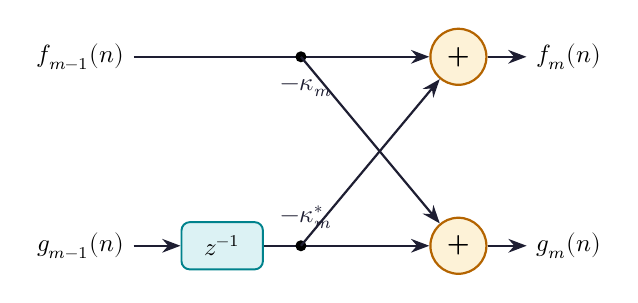
\begin{tikzpicture}[node distance=1.0cm and 1.5cm, every node/.style={font=\small}]
  % Nodes Left (Inputs)
  \node (f_in) at (0, 1.2) {$f_{m-1}(n)$};
  \node (g_in) at (0, -1.2) {$g_{m-1}(n)$};
  
  % Delay
  \node[block, text width=0.8cm, minimum height=0.6cm] (delay) at (1.8, -1.2) {$z^{-1}$};
  
  % Junctions
  \node[sumjunc] (sum_f) at (4.8, 1.2) {\textbf{+}};
  \node[sumjunc] (sum_g) at (4.8, -1.2) {\textbf{+}};
  
  % Tap points
  \coordinate (tap_f) at (2.8, 1.2);
  \coordinate (tap_g) at (2.8, -1.2);
  
  % Connections
  \draw[arrow] (g_in.east) -- (delay.west);
  \draw[line] (f_in.east) -- (tap_f);
  \draw[arrow] (tap_f) -- (sum_f.west);
  
  \draw[line] (delay.east) -- (tap_g);
  \draw[arrow] (tap_g) -- (sum_g.west);
  
  \fill (tap_f) circle (2pt);
  \fill (tap_g) circle (2pt);
  
  % Diagonal multiplier paths (criss-cross)
  \draw[arrow] (tap_f) -- node[pos=0.3, above left] {$-\kappa_m$} (sum_g);
  \draw[arrow] (tap_g) -- node[pos=0.3, below left] {$-\kappa_m^*$} (sum_f);
  
  % Outputs
  \node (f_out) at (6.2, 1.2) {$f_m(n)$};
  \node (g_out) at (6.2, -1.2) {$g_m(n)$};
  
  \draw[arrow] (sum_f.east) -- (f_out.west);
  \draw[arrow] (sum_g.east) -- (g_out.west);
\end{tikzpicture}
\end{tcolorbox}

% ===============================================================================
\section{Relationship with AR Modeling and Levinson-Durbin Recursion}
% ===============================================================================

An Autoregressive (AR) process of order $M$ is generated by filtering white noise through an all-pole filter. The AR parameters and reflection coefficients are equivalent representations of the same process.

\subsection{Levinson-Durbin Recursion}
It solves the Yule-Walker equations $\mathbf{R}\mathbf{a} = \mathbf{r}$ with $O(M^2)$ complexity instead of $O(M^3)$ matrix inversion. The recursion steps for order $m=1, 2, \dots, M$:
\begin{align}
  \Delta_{m-1} &= r(m) - \sum_{i=1}^{m-1} a_{m-1, i} r(m-i) \\
  \kappa_m &= \frac{\Delta_{m-1}}{E_{m-1}} \\
  a_{m, i} &= a_{m-1, i} - \kappa_m a_{m-1, m-i}^* \quad (i=1, \dots, m-1) \\
  a_{m, m} &= \kappa_m \\
  E_m &= E_{m-1}(1 - |\kappa_m|^2)
\end{align}
where $E_0 = r(0)$ is the input variance, and $\kappa_m$ is the reflection coefficient.

% ===============================================================================
\section{Joint Process Estimator and Gradient Adaptive Lattice}
% ===============================================================================

\subsection{Joint Process Estimator (JPE)}
The JPE uses the backward prediction errors $g_m(n)$ of a lattice predictor as the input to a transversal filter to estimate a desired signal $d(n)$. Because the backward errors $\{g_0(n), \dots, g_M(n)\}$ are mutually orthogonal, the estimator weights $h_m$ can be optimized independently:
\begin{equation}
  \hat{d}(n) = \sum_{m=0}^M h_m^* g_m(n), \quad h_m = \frac{\mathbb{E}[d(n)g_m^*(n)]}{\mathbb{E}[|g_m(n)|^2]}
\end{equation}

\subsection{Gradient Adaptive Lattice (GAL)}
GAL is the adaptive implementation of the lattice filter. The reflection coefficients $\kappa_m$ are updated recursively using a stochastic gradient approach:
\begin{align}
  D_m(n) &= \beta D_m(n-1) + (1-\beta) \left[ |f_m(n)|^2 + |g_m(n-1)|^2 \right] \\
  \kappa_{m+1}(n+1) &= \kappa_{m+1}(n) + \frac{\mu}{D_m(n)} \left[ f_m(n) g_m^*(n-1) \right]
\end{align}
where $\beta$ is a smoothing factor and $D_m(n)$ estimates the power at stage $m$.

\begin{tcolorbox}[examplebox, title={Example: Levinson-Durbin Recursion}]
Given autocorrelation values $r(0) = 1.0, r(1) = 0.5, r(2) = 0.125$. Run the Levinson-Durbin recursion to find the reflection coefficients $\kappa_1, \kappa_2$ and the predictor coefficients of a second-order predictor.

\textbf{Solution:}
Initialize: $E_0 = r(0) = 1.0$.
\textbf{Iteration 1 ($m=1$):}
\[
  \Delta_0 = r(1) = 0.5
\]
\[
  \kappa_1 = \frac{\Delta_0}{E_0} = \frac{0.5}{1.0} = 0.5
\]
Predictor coefficient:
\[
  a_{1,1} = \kappa_1 = 0.5
\]
Update error energy:
\[
  E_1 = E_0(1 - \kappa_1^2) = 1.0(1 - 0.25) = 0.75
\]
\textbf{Iteration 2 ($m=2$):}
\[
  \Delta_1 = r(2) - a_{1,1}r(1) = 0.125 - (0.5 \times 0.5) = 0.125 - 0.25 = -0.125
\]
\[
  \kappa_2 = \frac{\Delta_1}{E_1} = \frac{-0.125}{0.75} = -\frac{1}{6} \approx -0.1667
\]
Predictor coefficients:
\[
  a_{2,2} = \kappa_2 = -0.1667
\]
\[
  a_{2,1} = a_{1,1} - \kappa_2 a_{1,1} = 0.5 - \left(-\frac{1}{6} \times 0.5\right) = 0.5 + 0.0833 = 0.5833
\]
Update error energy:
\[
  E_2 = E_1(1 - \kappa_2^2) = 0.75 \left(1 - \frac{1}{36}\right) = 0.75 \times \frac{35}{36} = 0.7292
\]
The reflection coefficients are $\kappa_1 = 0.5, \kappa_2 = -0.1667$, and predictor coefficients are $a_{2,1} = 0.5833, a_{2,2} = -0.1667$.
\end{tcolorbox}

% ===============================================================================
% MANDATORY QUICK REVISION PAGE
% ===============================================================================
\newpage
\begin{center}
  {\large\bfseries\color{myred} Quick Revision --- Module IV}\\[3pt]
  {\small\color{mydark} Lattice Filters \& Linear Prediction $|$ PE-EC702A}
\end{center}
\noindent{\color{myred}\rule{\linewidth}{1.2pt}}
\vspace{4pt}

\begin{tcolorbox}[formulabox, title={\textbf{Key Formulas at a Glance}}]
\renewcommand{\arraystretch}{1.3}
\begin{tabularx}{\linewidth}{B{4.5cm} X}
Forward Error & $f_m(n) = f_{m-1}(n) - \kappa_m^* g_{m-1}(n-1)$ \\[6pt]
Backward Error & $g_m(n) = g_{m-1}(n-1) - \kappa_m f_{m-1}(n)$ \\[6pt]
Reflection Coeff. ($\kappa_m$) & $\kappa_m = \frac{2\mathbb{E}[f_{m-1}(n) g_{m-1}^*(n-1)]}{\mathbb{E}[|f_{m-1}(n)|^2] + \mathbb{E}[|g_{m-1}(n-1)|^2]}$ \\[6pt]
Levinson-Durbin $\kappa_m$ & $\kappa_m = \Delta_{m-1}/E_{m-1}$ \\[6pt]
Predictor Coefficient Update & $a_{m, i} = a_{m-1, i} - \kappa_m a_{m-1, m-i}^*$ \quad ($a_{m,m} = \kappa_m$) \\[6pt]
Error Energy Update & $E_m = E_{m-1}(1 - |\kappa_m|^2)$
\end{tabularx}
\end{tcolorbox}

\begin{tcolorbox}[defbox, title={\textbf{One-Line Definitions}}]
\begin{itemize}[leftmargin=*, itemsep=2.5pt, topsep=0pt]
  \item \textbf{Forward Prediction Error:} The difference between the current signal sample and its linear estimate based on past samples.
  \item \textbf{Backward Prediction Error:} The difference between a past signal sample and its estimate based on subsequent samples.
  \item \textbf{Reflection Coefficient:} The correlation metric $\kappa_m$ bounded in $[-1, 1]$ parameterizing a lattice stage.
  \item \textbf{Levinson-Durbin Recursion:} An efficient $O(M^2)$ recursive algorithm to solve the Yule-Walker equations.
  \item \textbf{Joint Process Estimator:} A structure utilizing orthogonal backward errors to estimate an external desired signal.
  \item \textbf{GAL Filter:} A gradient-based adaptive lattice filter that adjusts reflection coefficients stage-by-stage.
\end{itemize}
\end{tcolorbox}

\begin{tcolorbox}[exambox, title={\textbf{Frequently Asked / Viva Questions}}]
\begin{enumerate}[topsep=0pt, label=\textbf{Q\arabic*.}, itemsep=5pt]
  \item \Q{What are the initial conditions for the lattice filter recursions?}
    $f_0(n) = g_0(n) = x(n)$, representing the raw input sample.
  \item \Q{Explain why lattice filters are preferred in hardware over transversal (FIR) filters.}
    Lattice filters are modular. Increasing the filter order simply requires adding more identical stages at the end, without recalculating prior stages' coefficients.
  \item \Q{What condition must reflection coefficients satisfy to ensure system stability?}
    $|\kappa_m| < 1$ for all stages $m$. If any $|\kappa_m| \ge 1$, the corresponding synthesis filter becomes unstable.
  \item \Q{Why are backward prediction errors $g_m(n)$ orthogonal to each other?}
    Because $g_m(n)$ represents the component of $x(n-m)$ that is orthogonal to the subspace spanned by $\{x(n), \dots, x(n-m+1)\}$. Thus, $\mathbb{E}[g_i(n)g_j^*(n)] = 0$ for $i \ne j$.
  \item \Q{How does the computational complexity of Levinson-Durbin compare to direct matrix inversion?}
    Levinson-Durbin requires $O(M^2)$ operations, whereas direct inversion of the correlation matrix via Gaussian elimination requires $O(M^3)$ operations.
  \item \Q{What is the relationship between predictor coefficients and reflection coefficients?}
    Predictor coefficients $a_{M,k}$ are calculated from reflection coefficients $\kappa_m$ using the step-up recursion relation: $a_{m,i} = a_{m-1,i} - \kappa_m a_{m-1,m-i}^*$.
  \item \Q{What is a Joint Process Estimator (JPE)?}
    It is an adaptive structure that first orthogonalizes the input signal using a lattice filter, and then estimates a desired response by forming a weighted linear combination of the orthogonal backward prediction errors.
  \item \Q{Define the PARCOR coefficient.}
    It stands for PARTial CORrelation coefficient, which is mathematically identical to the reflection coefficient $\kappa_m$ in a lattice filter.
  \item \Q{Why does the error energy $E_m$ decrease with increase in predictor order $m$?}
    Because $E_m = E_{m-1}(1 - |\kappa_m|^2)$, and since $|\kappa_m| < 1$, the factor $(1 - |\kappa_m|^2) \le 1$, meaning adding more taps can only reduce (or keep equal) the prediction error power.
  \item \Q{What is the role of the power estimator $D_m(n)$ in the GAL algorithm?}
    It normalizes the step-size for each stage individually (similar to NLMS), ensuring that convergence speed is uniform across all stages regardless of local signal power.
\end{enumerate}
\end{tcolorbox}

\begin{tcolorbox}[tikzbox, title={Comparison of Transversal vs. Lattice Predictor Structures}]
\renewcommand{\arraystretch}{1.45}
\par\noindent
{\renewcommand{\arraystretch}{1.65}%
\begin{tabularx}{\linewidth}{|B{3.2cm}|Y|Y|}
\hline
\textbf{Property} & \textbf{Transversal (Tapped Delay Line)} & \textbf{Lattice Structure} \\
\hline
\textbf{Modularity} & Low (adding a tap changes all weights) & High (adding a tap is just adding a stage) \\[4pt]
\hline
\textbf{Stability Check} & Complex (requires finding roots of polynomial) & Simple (checks if $|\kappa_m| < 1$ for all stages) \\[4pt]
\hline
\textbf{Numerical Sensitivity} & High (sensitive to coefficient quantization) & Low (robust to finite word-length effects) \\[4pt]
\hline
\textbf{Complexity} & $O(M)$ multiplications per update & $O(M)$ multiplications per update (slightly higher constant) \\[4pt]
\hline
\end{tabularx}
}
\end{tcolorbox}

\end{document}
